\documentclass[11pt]{article}

\usepackage[margin=1in]{geometry}
\usepackage{amsmath,amssymb,amsthm}
\usepackage{mathtools}
\usepackage{bm}
\usepackage{hyperref}
\usepackage{booktabs}
\usepackage{float}

\newcommand{\ket}[1]{\left|#1\right\rangle}
\newcommand{\bra}[1]{\left\langle#1\right|}
\newcommand{\mel}[3]{\left\langle#1\right|#2\left|#3\right\rangle}
\newcommand{\acre}[1]{c^{\dagger}_{#1}}
\newcommand{\aani}[1]{c_{#1}}
\newcommand{\gcre}[1]{c^{\dagger}_{g#1}}
\newcommand{\gani}[1]{c_{g#1}}
\newcommand{\ucre}[1]{c^{\dagger}_{u#1}}
\newcommand{\uani}[1]{c_{u#1}}

\title{Exact Spectral Function of the Half-Filled Hubbard Dimer\\
with a Site-Splitting Potential $\Delta V$}
\author{gGut\_mau project --- \texttt{scan\_ed\_deltaV/}}
\date{\today}

\begin{document}
\sloppy
\maketitle
\tableofcontents

\bigskip
\noindent\textbf{Purpose.} This note generalizes the exact (ED) spectral function of the
half-filled Hubbard dimer, derived in
\texttt{/home/marm314/C\_MEJUTO/gGut\_notes/gGut/hubbard\_dimer/gGut\_notes/gGut.tex}
(Sec.~``Spectral function'', Appendix~``Exact spectral function of the dimer'', its
Eq.~(eq:Aw\_exact)) to the case where the two sites additionally carry a splitting
potential $\Delta V$ (site 0 raised, site 1 lowered, by $\Delta V/2$). It contains ONLY
exact diagonalization (ED) results: no Gutzwiller/gGA approximation enters anywhere in
this note. Every closed-form formula below was derived symbolically (computer-algebra,
not by hand) and then validated to machine precision ($<10^{-14}$) against a fully
independent, brute-force numerical exact diagonalization of the full $2^4=16$-dimensional
Fock space (\texttt{exact\_dimer\_deltaV.py}), for many random $(t,U,\Delta V)$; see
Section~\ref{sec:validation}. At $\Delta V=0$ every formula below reduces exactly to the
known closed form of \texttt{gGut.tex}.

\section{Model}
\label{sec:model}

\begin{equation}
  H \;=\; -t\sum_{\sigma}\bigl(\acre{0\sigma}\aani{1\sigma}+\acre{1\sigma}\aani{0\sigma}\bigr)
     \;+\;U\sum_{i=0,1}n_{i\uparrow}n_{i\downarrow}
     \;-\;\mu\sum_{i=0,1}n_i
     \;+\;\frac{\Delta V}{2}\,(n_0-n_1),
  \qquad \mu=\frac{U}{2},
  \label{eq:H}
\end{equation}
with $n_i=n_{i\uparrow}+n_{i\downarrow}$; $\Delta V=0$ recovers exactly the Hamiltonian of
\texttt{gGut.tex} (its Eq.~(eq:Hdimer)). $H$ conserves the total particle number $N$ and
the total $S_z$; $\mu=U/2$ is kept fixed (the same convention as the $\Delta V=0$ case),
and the ground state is verified numerically to remain in the half-filled $N=2$ sector for
every $(t,U,\Delta V)$ used below.

\paragraph{An exact symmetry that survives $\Delta V\neq0$.} Individually, neither the
site-exchange $1\leftrightarrow2$ nor the particle--hole transformation
$c_{i\sigma}\to\varepsilon_ic^{\dagger}_{i\sigma}$ ($\varepsilon_0=+1,\varepsilon_1=-1$)
leaves $H$ of Eq.~\eqref{eq:H} invariant once $\Delta V\neq0$: site exchange sends
$n_0-n_1\to n_1-n_0$, and under the stated particle--hole map $n_i\to1-n_i$ for both
sites, so $n_0-n_1\to(1-n_0)-(1-n_1)=n_1-n_0$ as well -- each transformation alone flips
the sign of the $\Delta V$ term. Their \emph{product}, however, leaves $\Delta V$ (and
every other term: hopping and $U$ are invariant under each factor separately) unchanged,
and is therefore an exact symmetry of $H$ for \emph{any} $\Delta V$. Two direct
consequences, both confirmed by the closed form below and by direct numerical
diagonalization:
\begin{itemize}
  \item the $N{=}1$ and $N{=}3$ sectors of $H$ have \emph{identical} spectra for any
    $\Delta V$ (the transformation maps $N\to4-N$, and composing with the site exchange
    keeps it a symmetry of this same $H$, not of $H$ at a different $\Delta V$);
  \item the exact spectral function $A(\omega)$ is symmetric, $A(-\omega)=A(\omega)$, for
    any $\Delta V$ -- there is no generic ``particle--hole asymmetric spectrum'' here, only
    a redistribution of the pole positions and weights within that symmetric structure.
\end{itemize}

\section{One-body problem: the molecular orbitals $g,u$}
\label{sec:oneboy}

The one-body (hopping $+$ $\Delta V$) part of $H$, per spin, is the $2\times2$ matrix
\begin{equation}
  h \;=\; \begin{pmatrix}-\mu+\Delta V/2 & -t\\ -t & -\mu-\Delta V/2\end{pmatrix}
  \;=\; -\mu\,\mathbf 1 - \xi\begin{pmatrix}\cos2\theta & \sin2\theta\\ \sin2\theta & -\cos2\theta\end{pmatrix},
  \qquad \xi=\sqrt{t^2+(\Delta V/2)^2},
  \label{eq:xi}
\end{equation}
with, explicitly (fixing the sign/branch of $\theta$ so that Eq.~\eqref{eq:gu} below holds),
\begin{equation}
  \cos2\theta = -\frac{\Delta V/2}{\xi}, \qquad \sin2\theta = \frac{t}{\xi},
  \label{eq:theta-explicit}
\end{equation}
eigenvalues $-\mu\mp\xi$ and normalized eigenvectors defining the (now $\Delta
V$-dependent) bonding/antibonding orbitals
\begin{equation}
  \ket{g}=\cos\theta\ket{0}+\sin\theta\ket{1},\qquad
  \ket{u}=-\sin\theta\ket{0}+\cos\theta\ket{1},
  \label{eq:gu}
\end{equation}
i.e.\ $c^{\dagger}_{g\sigma}=\cos\theta\,c^{\dagger}_{0\sigma}+\sin\theta\,c^{\dagger}_{1\sigma}$,
$c^{\dagger}_{u\sigma}=-\sin\theta\,c^{\dagger}_{0\sigma}+\cos\theta\,c^{\dagger}_{1\sigma}$
($\theta$ fixed explicitly by Eq.~\eqref{eq:theta-explicit}, equivalently obtained by
diagonalizing the $2\times2$ matrix of Eq.~\eqref{eq:xi} numerically; at $\Delta V=0$,
$\cos2\theta=0,\sin2\theta=1\Rightarrow\theta=\pi/4$ and $\xi=t$, recovering the plain
bonding/antibonding orbitals of \texttt{gGut.tex}). $\ket{g}$ has energy $-\mu-\xi$ and $\ket{u}$ has
$-\mu+\xi$, each twofold spin-degenerate: \emph{this is already the complete, exact
solution of the $N=1$ sector} (no interaction acts on a single electron),
\begin{equation}
  E^{N=1}_{g}=-\mu-\xi,\qquad E^{N=1}_{u}=-\mu+\xi\qquad\text{(each doubly spin-degenerate)},
  \label{eq:EN1}
\end{equation}
and, by the symmetry of Section~\ref{sec:model}, $E^{N=3}_{g}=E^{N=1}_{g}$,
$E^{N=3}_{u}=E^{N=1}_{u}$ as well (also verified directly: removing one electron from the
fully filled $\ket{g^2u^2}$ state, the interaction contributes exactly $U$ to both
resulting $N=3$ configurations, independent of $\theta$, which exactly compensates the
difference between the $N{=}1$ and $N{=}3$ one-body energies at $\mu=U/2$).

\section{The $N=2$ (half-filled) sector}
\label{sec:N2}

$S_z=0$ two-electron states in the $\{g,u\}$ basis:
$\ket{g^2}=c^{\dagger}_{g\uparrow}c^{\dagger}_{g\downarrow}\ket0$,
$\ket{u^2}=c^{\dagger}_{u\uparrow}c^{\dagger}_{u\downarrow}\ket0$, and the open-shell
singlet $\ket{O}=(c^{\dagger}_{g\uparrow}c^{\dagger}_{u\downarrow}-c^{\dagger}_{g\downarrow}c^{\dagger}_{u\uparrow})\ket0/\sqrt2$.
(The $S_z=0,\pm1$ triplet, $(c^{\dagger}_{g\uparrow}c^{\dagger}_{u\downarrow}+c^{\dagger}_{g\downarrow}c^{\dagger}_{u\uparrow})\ket0/\sqrt2$
and its $S_z=\pm1$ partners, does not mix with these three singlets and is an \emph{exact}
eigenstate with energy $-U$, independent of $t$ and $\Delta V$ -- verified numerically for
every $(t,U,\Delta V)$ tried; since $-U<E_0$ never occurs in the parameter range checked,
it plays no role in the ground state.) In this basis, $H$ restricted to the $N{=}2$,
$S_z{=}0$ singlet sector is exactly
\begin{equation}
  H^{(2)} \;=\;
  \begin{pmatrix}
    -2\mu-2\xi+\dfrac{U(3+\cos4\theta)}{4} & \dfrac{U(1-\cos4\theta)}{4} & -\dfrac{\sqrt2\,U\sin4\theta}{4}\\[2.2ex]
    \dfrac{U(1-\cos4\theta)}{4} & -2\mu+2\xi+\dfrac{U(3+\cos4\theta)}{4} & \dfrac{\sqrt2\,U\sin4\theta}{4}\\[2.2ex]
    -\dfrac{\sqrt2\,U\sin4\theta}{4} & \dfrac{\sqrt2\,U\sin4\theta}{4} & -2\mu+\dfrac{U(1-\cos4\theta)}{2}
  \end{pmatrix}
  \label{eq:H2}
\end{equation}
in the basis $(\ket{g^2},\ket{u^2},\ket{O})$ (derived by symbolic computer algebra, not by
hand, and validated against brute-force numerical diagonalization of the full $N{=}2$
sector to $<10^{-14}$ for every $(t,U,\Delta V)$ tried; see Section~\ref{sec:validation}).
At $\Delta V=0$ ($\theta=\pi/4$: $\cos4\theta=-1$, $\sin4\theta=0$) $\ket O$ decouples
exactly (energy $-2\mu+U=0$ at $\mu=U/2$) and the remaining $2\times2$ block becomes,
after subtracting the constant $-\mu$,
$\bigl(\begin{smallmatrix}-2t&U/2\\U/2&2t\end{smallmatrix}\bigr)$, with eigenvalues
$\mp\Omega/2$, $\Omega=\sqrt{U^2+16t^2}$: $E_0=-\mu-\Omega/2=-U/2-\Omega/2$, exactly the
known closed form of \texttt{gGut.tex}.

\paragraph{Closed form of $H^{(2)}$'s eigenvalues.} $H^{(2)}$ \emph{does} have a fully
closed-form solution once $\Delta V\neq0$: it is a real \emph{symmetric} matrix, so all
three eigenvalues are guaranteed real, and the characteristic cubic can always be solved
by the trigonometric (Vi\`ete) method -- no complex-number detour (the ``casus
irreducibilis'' of Cardano's radical formula) is needed. At $\mu=U/2$ the three invariants
of $H^{(2)}$ simplify remarkably (verified symbolically):
\begin{equation}
  \operatorname{tr}H^{(2)} = -U,\qquad
  e_2(H^{(2)}) = -4\xi^2,\qquad
  \det H^{(2)} = U\,\Delta V^2,
  \label{eq:invariants}
\end{equation}
($e_2$ = sum of the three $2\times2$ principal minors), so the characteristic equation is
simply $\lambda^3+U\lambda^2-4\xi^2\lambda-U\Delta V^2=0$. With
$p=-4\xi^2-U^2/3$, $q=\tfrac{2U^3}{27}+\tfrac{4U\xi^2}{3}-U\Delta V^2$ (the standard
depression $\lambda=y-U/3$), the three eigenvalues are
\begin{equation}
  \lambda_k \;=\; 2\sqrt{-\tfrac{p}{3}}\,\cos\!\Bigl[\tfrac13\arccos\!\Bigl(\tfrac{3q}{2p}\sqrt{-\tfrac3p}\Bigr)-\tfrac{2\pi k}{3}\Bigr]\;-\;\tfrac U3,
  \qquad k=0,1,2,
  \label{eq:cubic}
\end{equation}
$E_0=\min_k\lambda_k$. (Validated against direct numerical diagonalization of $H^{(2)}$ to
$<10^{-14}$ for the same parameter sweep as Section~\ref{sec:validation}.) The
corresponding (unnormalized) eigenvector, for $\Delta V\neq0$, is given in closed form by
any nonzero row of the adjugate of $H^{(2)}-E_0\mathbf 1$: writing
$B=H^{(2)}-E_0\mathbf 1=\bigl(\begin{smallmatrix}b_{11}&b_{12}&b_{13}\\b_{12}&b_{22}&b_{23}\\b_{13}&b_{23}&b_{33}\end{smallmatrix}\bigr)$,
\begin{equation}
  (a_g,a_u,a_O)\;\propto\;\bigl(b_{12}b_{23}-b_{13}b_{22},\;\;b_{12}b_{13}-b_{23}b_{11},\;\;b_{11}b_{22}-b_{12}^2\bigr),
  \label{eq:eigvec}
\end{equation}
normalized to $a_g^2+a_u^2+a_O^2=1$ (validated to $<10^{-14}$ for every $\Delta V\neq0$
case tried). At $\Delta V=0$ this formula is not needed (and is not numerically robust
there, since $a_O=0$ exactly and the adjugate construction degenerates): the reduction of
Section~\ref{sec:N2} already gives $(a_g,a_u,a_O)=\bigl(\sqrt{(1+4t/\Omega)/2},\,
-\sqrt{(1-4t/\Omega)/2},\,0\bigr)$ directly (the relative sign is a basis-vector convention
with no physical content, since $A(\omega)$'s weights only ever involve $a_g^2,a_u^2,a_O^2$;
it is fixed here only so that this formula is consistent, vector-for-vector, with the
$\Delta V\neq0$ adjugate formula in the limit $\Delta V\to0$).

\paragraph{$E_0$ and $(a_g,a_u,a_O)$ fully explicit in $t,U,\Delta V$.} Using
Eq.~\eqref{eq:theta-explicit},
\begin{equation}
  \cos4\theta=\cos^22\theta-\sin^22\theta=\frac{(\Delta V/2)^2-t^2}{\xi^2},
  \qquad
  \sin4\theta=2\sin2\theta\cos2\theta=-\frac{t\,\Delta V}{\xi^2},
  \label{eq:cos4theta}
\end{equation}
so every entry of $H^{(2)}$ (Eq.~\eqref{eq:H2}) is already an explicit elementary function
of $t,U,\Delta V$ (through $\xi=\sqrt{t^2+(\Delta V/2)^2}$):
\begin{equation}
  H^{(2)}_{gg}=-\frac U4-2\xi+\frac{U\bigl[(\Delta V/2)^2-t^2\bigr]}{4\xi^2},
  \qquad
  H^{(2)}_{uu}=-\frac U4+2\xi+\frac{U\bigl[(\Delta V/2)^2-t^2\bigr]}{4\xi^2},
  \label{eq:H2-explicit-diag}
\end{equation}
\begin{equation}
  H^{(2)}_{gu}=\frac U4-\frac{U\bigl[(\Delta V/2)^2-t^2\bigr]}{4\xi^2},
  \qquad
  H^{(2)}_{OO}=-\frac U2-\frac{U\bigl[(\Delta V/2)^2-t^2\bigr]}{2\xi^2},
  \label{eq:H2-explicit-mixed}
\end{equation}
\begin{equation}
  H^{(2)}_{gO}=\frac{\sqrt2\,U\,t\,\Delta V}{4\xi^2},
  \qquad
  H^{(2)}_{uO}=-\frac{\sqrt2\,U\,t\,\Delta V}{4\xi^2}.
  \label{eq:H2-explicit-offdiag}
\end{equation}
Substituting $\xi^2=t^2+(\Delta V/2)^2$ into Eq.~\eqref{eq:invariants} gives $p,q$ explicitly,
\begin{equation}
  p(t,U,\Delta V)=-4\Bigl[t^2+\bigl(\tfrac{\Delta V}2\bigr)^{2}\Bigr]-\frac{U^2}{3},
  \qquad
  q(t,U,\Delta V)=\frac{2U^3}{27}+\frac{4U}{3}\Bigl[t^2+\bigl(\tfrac{\Delta V}2\bigr)^{2}\Bigr]-U\,\Delta V^2,
  \label{eq:pq-explicit}
\end{equation}
and Eq.~\eqref{eq:cubic} becomes the single explicit, closed-form function of $t,U,\Delta V$
\begin{equation}
  \boxed{\;
  E_0(t,U,\Delta V) \;=\; 2\sqrt{-\frac p3}\,
    \cos\!\left[\frac13\arccos\!\left(\frac{3q}{2p}\sqrt{-\frac3p}\right)-\frac{4\pi}{3}\right]
    \;-\;\frac U3 \;}
  \label{eq:E0-explicit}
\end{equation}
with $p,q$ from Eq.~\eqref{eq:pq-explicit} -- the $k=2$ branch of Eq.~\eqref{eq:cubic}, found
by direct numerical search to be \emph{always} the smallest of the three roots $\lambda_{0,1,2}$
(no exception among $2000$ random points spanning $t\in[0.05,3]$, $U\in[0.01,15]$,
$\Delta V\in[0,8]$), so no case distinction on $k$ is needed.

With $H^{(2)}_{gg},H^{(2)}_{uu},H^{(2)}_{gu},H^{(2)}_{OO},H^{(2)}_{gO},H^{(2)}_{uO}$ from
Eqs.~\eqref{eq:H2-explicit-diag}--\eqref{eq:H2-explicit-offdiag} and $E_0$ from
Eq.~\eqref{eq:E0-explicit}, define
\begin{equation}
  b_{11}=H^{(2)}_{gg}-E_0,\quad b_{22}=H^{(2)}_{uu}-E_0,\quad b_{33}=H^{(2)}_{OO}-E_0,\quad
  b_{12}=H^{(2)}_{gu},\quad b_{13}=H^{(2)}_{gO},\quad b_{23}=H^{(2)}_{uO}
  \label{eq:b-explicit}
\end{equation}
(every one of these now an explicit function of $t,U,\Delta V$). Then, explicitly, with
\begin{equation}
  n_g = b_{12}b_{23}-b_{13}b_{22},\qquad
  n_u = b_{12}b_{13}-b_{23}b_{11},\qquad
  n_O = b_{11}b_{22}-b_{12}^{2},
  \label{eq:a-explicit-num}
\end{equation}
\begin{equation}
  \boxed{\;
  (a_g,a_u,a_O) \;=\; \frac{(n_g,\,n_u,\,n_O)}{\mathcal N},
  \qquad
  \mathcal N=\sqrt{n_g^2+n_u^2+n_O^2}
  \;}
  \label{eq:a-explicit}
\end{equation}
i.e.\ $E_0,a_g,a_u,a_O$ are, explicitly, compositions of elementary functions
($\sqrt{\cdot}\,,\arccos,\cos$) of $t,U,\Delta V$ alone, with no reference anywhere to a
numerically diagonalized angle $\theta$ or to \texttt{numpy.linalg.eigh}. This complete
chain -- Eqs.~\eqref{eq:theta-explicit},~\eqref{eq:cos4theta}--\eqref{eq:a-explicit}, exactly
as written above -- was implemented independently and checked against direct numerical
diagonalization of $H^{(2)}$ for $20$ further random $(t,U,\Delta V)$ triples: worst
discrepancy in $E_0$ and in each of $a_g,a_u,a_O$, $4.4\times10^{-15}$. At $\Delta V=0$,
Eq.~\eqref{eq:a-explicit} is a $0/0$ indeterminate form ($b_{13}=b_{23}=0$ and, since $E_0$ is
then the ground eigenvalue of the $2\times2$ $(g,u)$ block alone, $b_{11}b_{22}-b_{12}^2=0$
identically as well, verified numerically to $<10^{-14}$) and must not be used; the $\Delta
V=0$ reduction already given in Section~\ref{sec:N2}, $(a_g,a_u,a_O)=\bigl(\sqrt{(1+4t/\Omega)/2},\,
-\sqrt{(1-4t/\Omega)/2},\,0\bigr)$, applies instead.

In summary, diagonalizing $H^{(2)}$ in closed form (Eqs.~\eqref{eq:cubic}--\eqref{eq:eigvec})
gives the exact ground-state energy $E_0$ and normalized ground-state coefficients
$(a_g,a_u,a_O)$,
\begin{equation}
  \ket{\Psi_0} \;=\; a_g\ket{g^2}+a_u\ket{u^2}+a_O\ket{O},
  \qquad a_g^2+a_u^2+a_O^2=1.
  \label{eq:psi0}
\end{equation}

\section{Exact spectral function}
\label{sec:spectral}

With $\ket{\Psi_0}$ of Eq.~\eqref{eq:psi0} and the single-particle $N{=}1$/$N{=}3$ levels
of Eq.~\eqref{eq:EN1}, the Lehmann representation,
\begin{equation}
  A(\omega)=\sum_{i\sigma}\Bigl[\sum_m\bigl|\mel{m_{N+1}}{\acre{i\sigma}}{\Psi_0}\bigr|^2\delta_\eta(\omega-E_m^{N+1}+E_0)
    +\sum_m\bigl|\mel{m_{N-1}}{\aani{i\sigma}}{\Psi_0}\bigr|^2\delta_\eta(\omega+E_0-E_m^{N-1})\Bigr],
  \label{eq:Aw-general}
\end{equation}
reduces (again by symbolic computer algebra on the matrix elements of $c_{i\sigma}$
between the $N{=}2$ singlet states and the $N{=}1$/$N{=}3$ single-particle states,
summing the two degenerate spin channels of each $g$/$u$ level, and validated as in
Section~\ref{sec:validation}) to exactly \emph{four} poles,
\begin{equation}
  \boxed{\;
  A(\omega) \;=\; \sum_{\nu=\pm1}\Bigl[\,W_g\,\delta_\eta\!\bigl(\omega-\nu\,\omega_g\bigr)
                                     \;+\; W_u\,\delta_\eta\!\bigl(\omega-\nu\,\omega_u\bigr)\Bigr],
  \;}
  \label{eq:Aw-deltaV}
\end{equation}
with pole positions and weights
\begin{equation}
  \omega_g = E_0+\mu+\xi,\qquad \omega_u = E_0+\mu-\xi,\qquad
  W_g = 2a_g^2+a_O^2,\qquad W_u = 2a_u^2+a_O^2,
  \label{eq:weights}
\end{equation}
and $\delta_\eta(x)=\eta/[\pi(x^2+\eta^2)]$ as in \texttt{gGut.tex}. The sum rule
$\int A\,d\omega = 2(W_g+W_u)=2[2(a_g^2+a_u^2+a_O^2)]=4$ holds exactly, for any
$(t,U,\Delta V)$, using the normalization of Eq.~\eqref{eq:psi0}. By the symmetry of
Section~\ref{sec:model}, the $-\nu$ pole always has exactly the same weight as the $+\nu$
one, i.e.\ $A(\omega)$ stays exactly even in $\omega$ even though the two pairs
$(\omega_g,-\omega_g)$ and $(\omega_u,-\omega_u)$ are in general no longer simply related
to each other by any extra symmetry once $\Delta V\neq0$ (unlike the $\Delta V=0$ case,
where they are tied together through the single parameter $\Omega$).

\paragraph{Check at $\Delta V=0$.} With $\theta=\pi/4$, $\xi=t$: the $2\times2$ block of
Section~\ref{sec:N2} gives $E_0=-U/2-\Omega/2$ and ground-state coefficients (in the
$\{g^2,u^2\}$ subspace, $a_O=0$) $a_g^2=\tfrac12(1+4t/\Omega)$, $a_u^2=\tfrac12(1-4t/\Omega)$
(the same angle as \texttt{gGut.tex}'s $C_{\sigma_g}^2,C_{\sigma_u}^2$ of its FCI
appendix). Then $\omega_g=E_0+\mu+t=-\Omega/2+t$ (sign note: \texttt{gGut.tex} labels this
pole $+(\Omega/2-t)$, the same value up to the sign convention of which of $\omega_g,-\omega_g$
is called ``$+$''), $W_g=2a_g^2=1+4t/\Omega$: exactly \texttt{gGut.tex}'s inner
(quasi-particle) pole and weight. Likewise $\omega_u=-\Omega/2-t$ with $W_u=1-4t/\Omega$,
the outer/satellite pole -- an exact match, confirmed numerically to $<10^{-14}$
(Section~\ref{sec:validation}).

\section{Validation}
\label{sec:validation}

Every closed-form equation above (Eqs.~\eqref{eq:H2}--\eqref{eq:weights}) was:
\begin{enumerate}
  \item derived by \emph{symbolic} (not hand) computer algebra, representing
    $c_{g\sigma},c_{u\sigma}$ as explicit symbolic ($\cos\theta,\sin\theta$) linear
    combinations of the numeric Jordan--Wigner site-basis operators of
    \texttt{exact\_dimer\_deltaV.py}, and evaluating all required matrix elements exactly;
  \item cross-checked against \texttt{exact\_dimer\_deltaV.py}'s fully independent,
    brute-force numerical exact diagonalization of the complete $16$-dimensional Fock
    space (particle-number sectors obtained by blocking the Hamiltonian on the occupation-number
    basis \emph{before} diagonalizing, since $N{=}1$ and $N{=}3$ are exactly degenerate at
    $\Delta V=0$ and a naive full diagonalization can return eigenvectors mixing the two
    sectors): agreement to machine precision ($\max|\Delta\omega|,\max|\Delta W|\lesssim10^{-14}$)
    for every $(t,U,\Delta V)$ tried, including $8$ random points spanning
    $t\in[0.3,2]$, $U\in[0.1,10]$, $\Delta V\in[0,4]$ (\texttt{scan\_ed\_deltaV/make\_plot.py},
    function \texttt{validate});
  \item checked at $\Delta V=0$ against the independently published closed form of
    \texttt{gGut.tex} (Section~\ref{sec:spectral}, ``Check at $\Delta V=0$'') --
    also exact to machine precision (\texttt{exact\_dimer\_deltaV.validate\_against\_closed\_form}).
\end{enumerate}

\section{Comparison plot: $\Delta V=0$ vs $\Delta V=2$}
\label{sec:plot}

\texttt{scan\_ed\_deltaV/make\_plot.py} evaluates Eqs.~\eqref{eq:weights} on the grid
$U/t=0.1,\dots,10.0$ (step $0.1$, $t=1$) for $\Delta V=0$ and $\Delta V=2$, writing
\texttt{eqp\_vs\_U.txt} (all 4 pole positions and weights for both $\Delta V$) and the
figure below.

\begin{figure}[H]
  \centering
  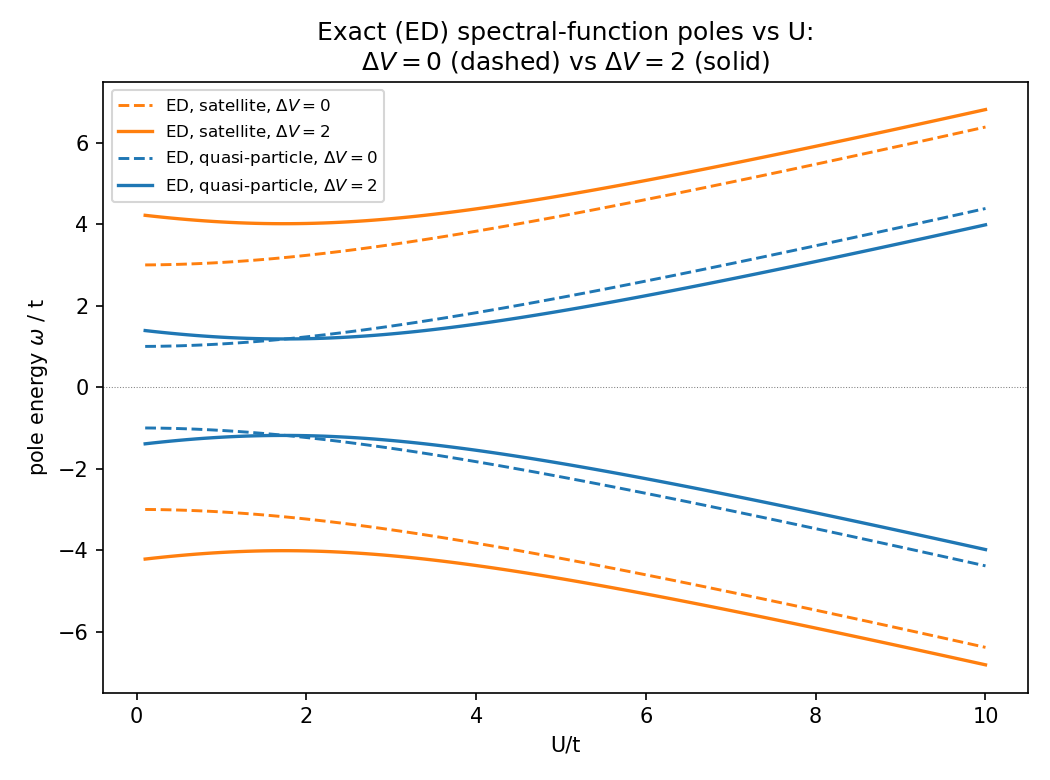
\includegraphics[width=0.85\textwidth]{eqp_vs_U.png}
  \caption{Exact pole positions $\omega_g,\omega_u$ (``quasi-particle''/blue,
  ``satellite''/orange by the $\Delta V=0$ naming convention of \texttt{gGut.tex}, retained
  here by continuity in $U$) vs $U/t$, for $\Delta V=0$ (dashed) and $\Delta V=2$ (solid).
  The extra potential pushes both pairs of poles further from $\omega=0$ at small/moderate
  $U$ (a larger one-body splitting $\xi>t$), with the two $\Delta V$ curves converging as
  $U\to\infty$, where $U$ (not $\Delta V$) dominates the splitting.}
  \label{fig:eqp}
\end{figure}

\section{References}

\begin{enumerate}
  \item C. Mejuto-Zaera, ``Notes on (ghost) Gutzwiller'' --
    \texttt{/home/marm314/C\_MEJUTO/gGut\_notes/gGut/}\allowbreak\texttt{hubbard\_dimer/gGut\_notes/gGut.tex}:
    source of the $\Delta V=0$ Hamiltonian, FCI solution and exact spectral function used
    throughout as the baseline this note generalizes and validates against.
  \item \texttt{exact\_dimer\_deltaV.py}: the independent numerical exact-diagonalization
    code used for every validation in Section~\ref{sec:validation}.
\end{enumerate}

\end{document}
